\documentclass[scheme = chinese]{ctexart}

% Set page size and margins
% Replace `letterpaper' with`a4paper' for UK/EU standard size
\usepackage[a4paper,top=2cm,bottom=2cm,left=3cm,right=3cm,marginparwidth=1.75cm]{geometry}
% Useful packages
\usepackage{amsmath}
\usepackage{graphicx}
\usepackage[colorlinks=false, allcolors=blue]{hyperref}
\usepackage[final]{pdfpages}
\usepackage{booktabs}
\usepackage{caption}
\usepackage{makecell}
\graphicspath{ {./images/} }
\newcommand*{\fullref}[1]{\hyperref[{#1}]{第 \pageref*{#1} 页:\autoref*{#1} \nameref*{#1}}} % One single link
\usepackage{varioref}
\usepackage{float}
\usepackage{listings}
\usepackage{minted}
\usepackage{subfiles}

\begin{document}
\title{MIPS单周期CPU开发}
\author{孙天天 19071110}
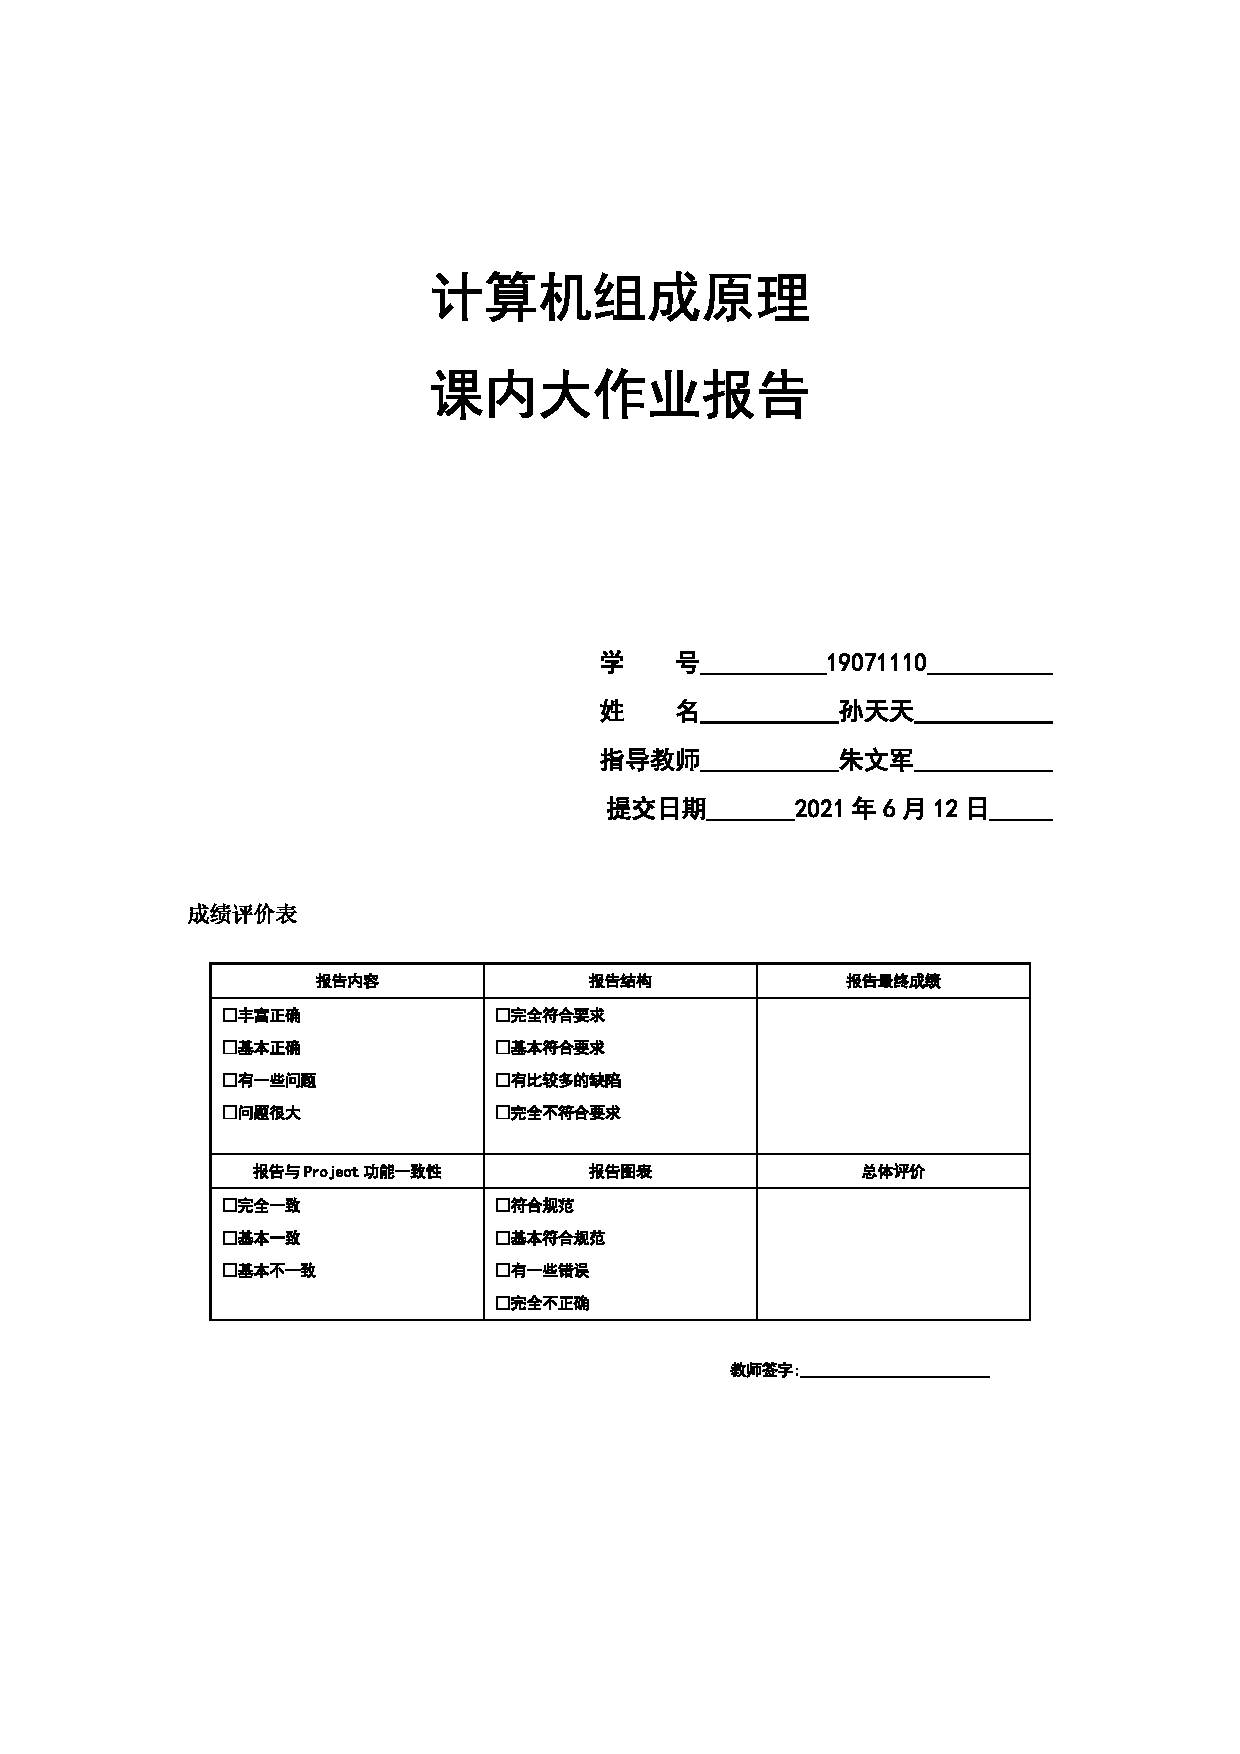
\includepdf[pages=-,pagecommand={},width=\textwidth]{cover.pdf}

\tableofcontents
\clearpage

\maketitle

\subfile{section1-overall.tex}
\clearpage
\subfile{section2-modules.tex}
\clearpage
\subfile{section3-testing.tex}
\clearpage

\section{总结与收获}


\end{document}